\chapter{页表}\label{ch03}

页表是最流行的帮助操作系统为每个进程提供私有地址空间和内存的机制。
页表决定了内存地址的含义和哪些物理内存可以被进程访问。
这允许xv6隔离开不同进程的地址空间并复用同一个物理内存。
页表是一个很流行的设计,因为它们提供了一个间接层,操作系统可以利用这个间接层实现一些技巧。
xv6也使用了一些技巧:把相同的内存(一个trampoline页)映射到多个地址空间中、使用一个未映射的页来保护内核和用户栈。
本章的其余部分解释了RISC-V硬件提供的页表以及xv6如何使用它们。

\section{页表硬件}
提醒一下,RISC-V指令(用户空间和内核空间都是)操作虚拟地址。
机器的RAM,或者说物理内存,是通过物理地址索引的。
RISC-V页表硬件负责连接这两种地址,它把每个虚拟地址映射到物理地址。

xv6在Sv39 RISC-V上运行,意思是只有64位虚拟地址的低39位才会被用到,高25位不使用。
在Sv39配置中,一个RISC-V页表在逻辑上是一个长度为$2^{27}$(134,217,728)的\emph{页表项(page table entries, PTEs)}的数组。
每一个PTE都包含一个44位的物理页号(PPN)和一些标记。
分页硬件在翻译虚拟地址时首先使用39位中的高27位去索引页表,得到一个PTE,然后用其中44位的PPN和39位中的低12位拼接出一个56位的物理地址。
\autoref{f3-1}展示了这个过程,图中简单把页表看做一个PTE的数组(完整的流程见\autoref{f3-2})。
页表允许操作系统以4096($2^{12}$)字节对齐的块为粒度控制虚拟到物理地址的翻译。
这样的一个块被称为一个\emph{页(page)}。

\begin{figure}[htbp]
    \centering
    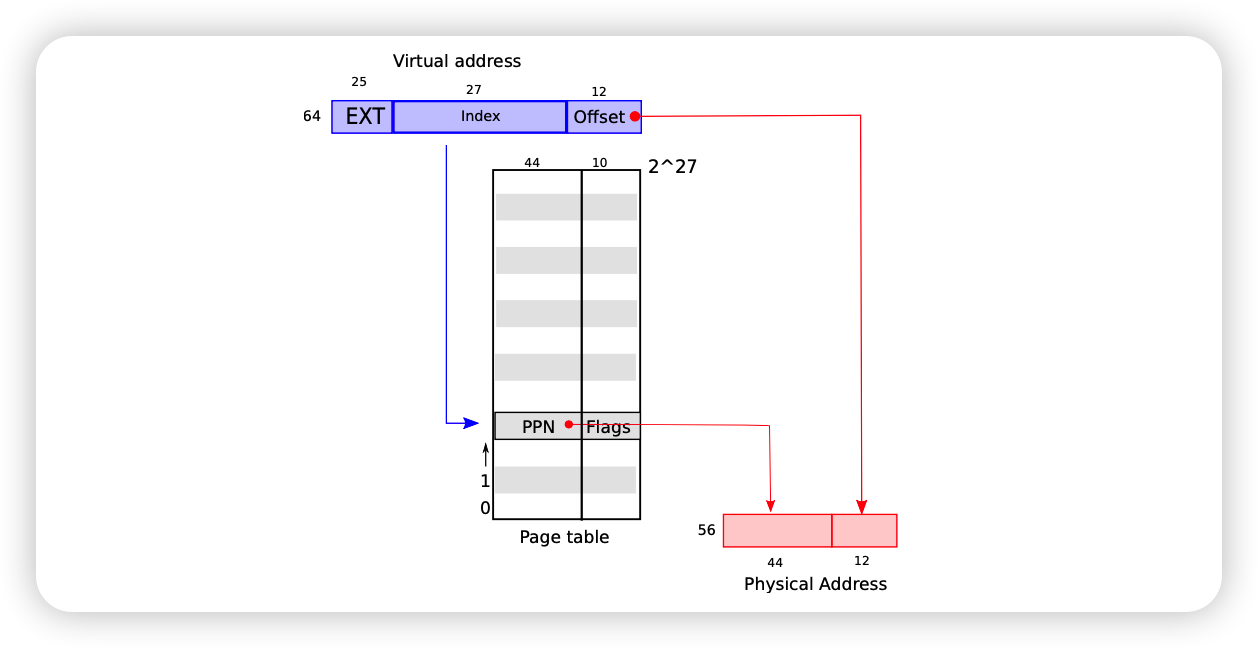
\includegraphics[width=0.8\textwidth]{../imgs/f3-1.png}
    \caption{RISC-V虚拟和物理地址(简化的逻辑页表)}
    \label{f3-1}
\end{figure}

\begin{figure}[htbp]
    \centering
    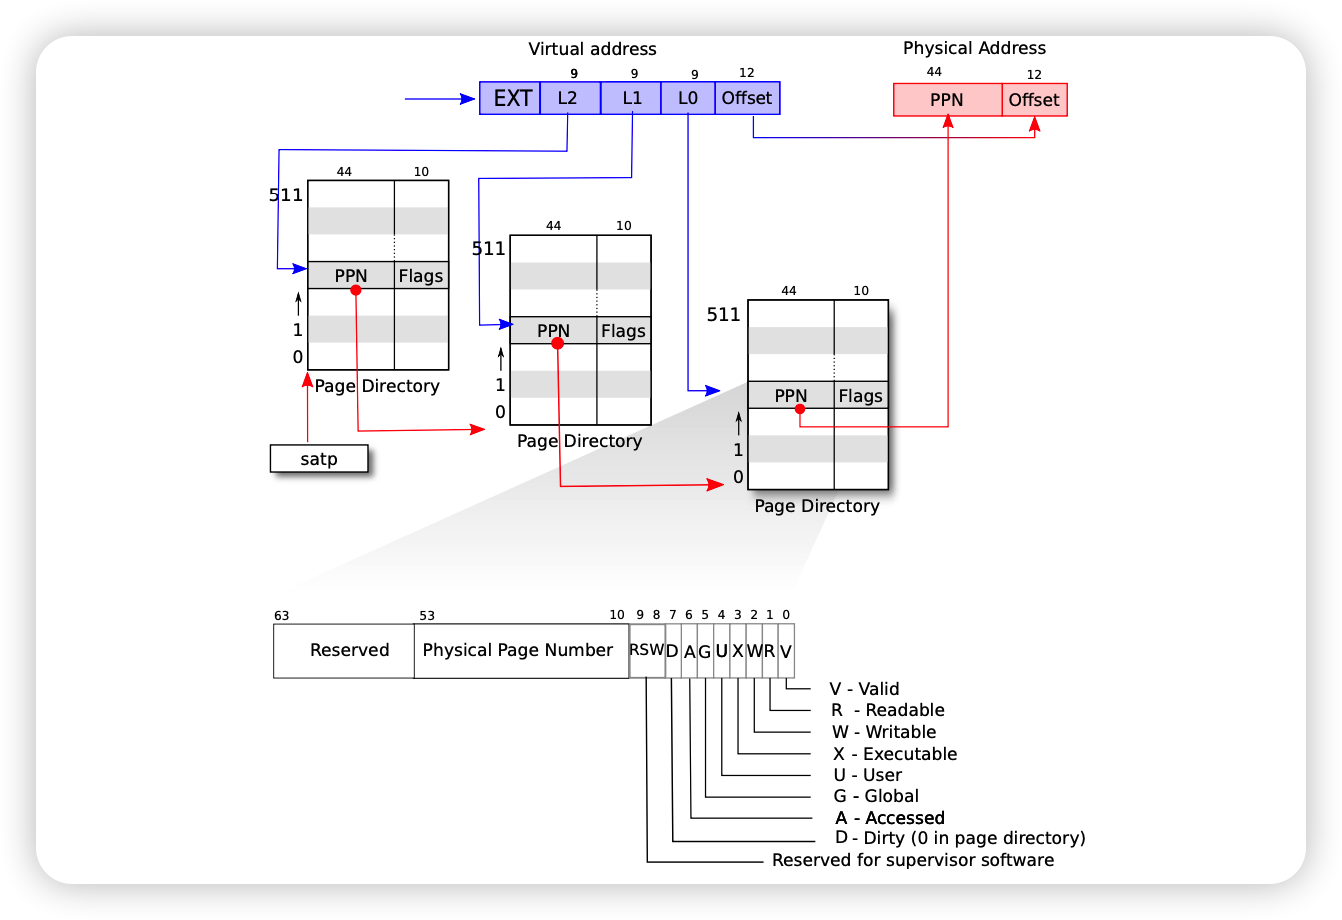
\includegraphics[width=0.8\textwidth]{../imgs/f3-2.png}
    \caption{RISC-V地址翻译细节}
    \label{f3-2}
\end{figure}

在Sv39 RISC-V中,虚拟地址的高25位不用于翻译。
物理地址也还有增长的空间:PTE的格式中还有空间可以让物理页号再增长10位。
RISC-V的设计者根据技术预测选择了这些数字。
$2^{39}$个字节也就是512GB的虚拟地址空间对于运行在RISC-V计算机中的应用来说应该足够了。
$2^{56}$的物理地址空间在不久的未来都足够容纳很多I/O设备和DRAM芯片。
如果还需要更大的空间,RISC-V的设计者还定义了48位虚拟地址的Sv48[3]。

如\autoref{f3-2}所示,一个RISC-V CPU用3步把一个虚拟地址翻译成物理地址。
页表以3级树的形式被存储在物理内存中。
树的根是一个4096字节的页表,它包含512个PTE,每个PTE中都包含了一个下一级页表的物理地址。
每个第二级页表都包含了512个PTE,每个PTE中都包含了树的最后一级。
分页硬件使用27位中的最高9位在根页表中选择一个PTE,用中间9位在第二级页表中选择一个PTE,用低9位去选择最终的PTE。(在Sv48 RISC-V中一个页表有4级,虚拟地址的第39到47位用来在顶级页表索引。)

如果翻译地址所需的三个PTE中的任何一个不存在,分页硬件会抛出一个\emph{页面错误异常(page-fault exception)},让内核来处理这个异常(见\autoref{ch04})。

\autoref{f3-2}中的3级架构与\autoref{f3-1}中的单级设计相比,可以用一种更加内存高效地方式记录PTE。
在通常情况下很大范围内的虚拟地址都没有映射,三级结构可以省略整个页面目录。
例如,如果一个应用只使用了从0开始的很少的页,那么顶级页表的1到511号表项都是无效的,因此kernel不需要为511个中间的页表分配页面。
因此,在这个例子中,3级的设计节省了511个中间的页表和$511 \times 512$个底级页表。

虽然CPU在执行load/store指令时在硬件中运行三级结构,但这种3级架构的一个潜在缺点是在执行load/store指令时CPU必须从内存中加载3个PTE才能把虚拟地址翻译到物理地址。
为了避免从物理内存中加载PTE的开销,RISC-V CPU会把页表项缓存在\emph{翻译查找缓冲区(Translation Look-aside Buffer, TLB)}中。

每个PTE都包含一些标注位,它们告诉分页硬件该虚拟地址允许的操作。
\texttt{PTE\_V}指示PTE是否存在:如果该位未被设置,那么引用对应的页面会导致异常(即不允许)。
\texttt{PTE\_R}控制指令是否可以读取该页。
\texttt{PTE\_W}控制指令是否可以写入该页。
\texttt{PTE\_X}控制指令是否可以把页的内容解释为指令并执行它们。
\texttt{PTE\_U}控制用户模式下的指令是否可以访问该页;如果\texttt{PTE\_U}未被设置,该PTE只能在管理模式下使用。
\autoref{f3-2}展示了所有这些位的含义。
这些标记和所有其他分页硬件相关的结构体定义在\href{https://github.com/mit-pdos/xv6-riscv/blob/risc/kernel/riscv.h}{(kernel/riscv.h)}。

为了让CPU使用页表,内核必须把根页表的物理地址写入\texttt{satp}寄存器。
执行后续的指令时CPU会使用\texttt{satp}指向的页表来翻译所有的地址。
每个CPU都有自己的\texttt{satp},所以不同的CPU可以运行不同的进程,每个进程都有自己的页表所描述的地址空间。

通常内核会把所有物理内存都映射进它的页表里,这样它可以使用load/store指令读取和写入任何物理内存位置。
因为页面目录也在物理内存中,内核可以通过使用标准store指令写入PTE的虚拟地址来编程页面目录中PTE的内容。

解释一下相关的术语。
物理内存是指DRAM的存储单元。
物理内存中的每个字节都有一个地址,称为物理地址。
指令只使用虚拟地址,分页硬件把它翻译成物理地址,然后发送给DRAM硬件以读取或写入存储。
与物理内存和虚拟地址不同,虚拟内存并不是一个物理对象,而是指内核提供的管理物理内存和虚拟地址的抽象和机制的集合。

\section{内核地址空间}
xv6为每个进程维护一个描述用户地址空间的页表,还维护了一个唯一的描述内核地址空间的页表。
内核会设置它的地址空间的布局以让它能访问物理内存和特定虚拟地址处的各种硬件资源。
\autoref{f3-3}展示了怎么把内核虚拟地址映射到物理地址。
文件\href{URL}{(kernel/memlayout.h)}声明了xv6的内核内存布局中的常量。

\begin{figure}[htbp]
    \centering
    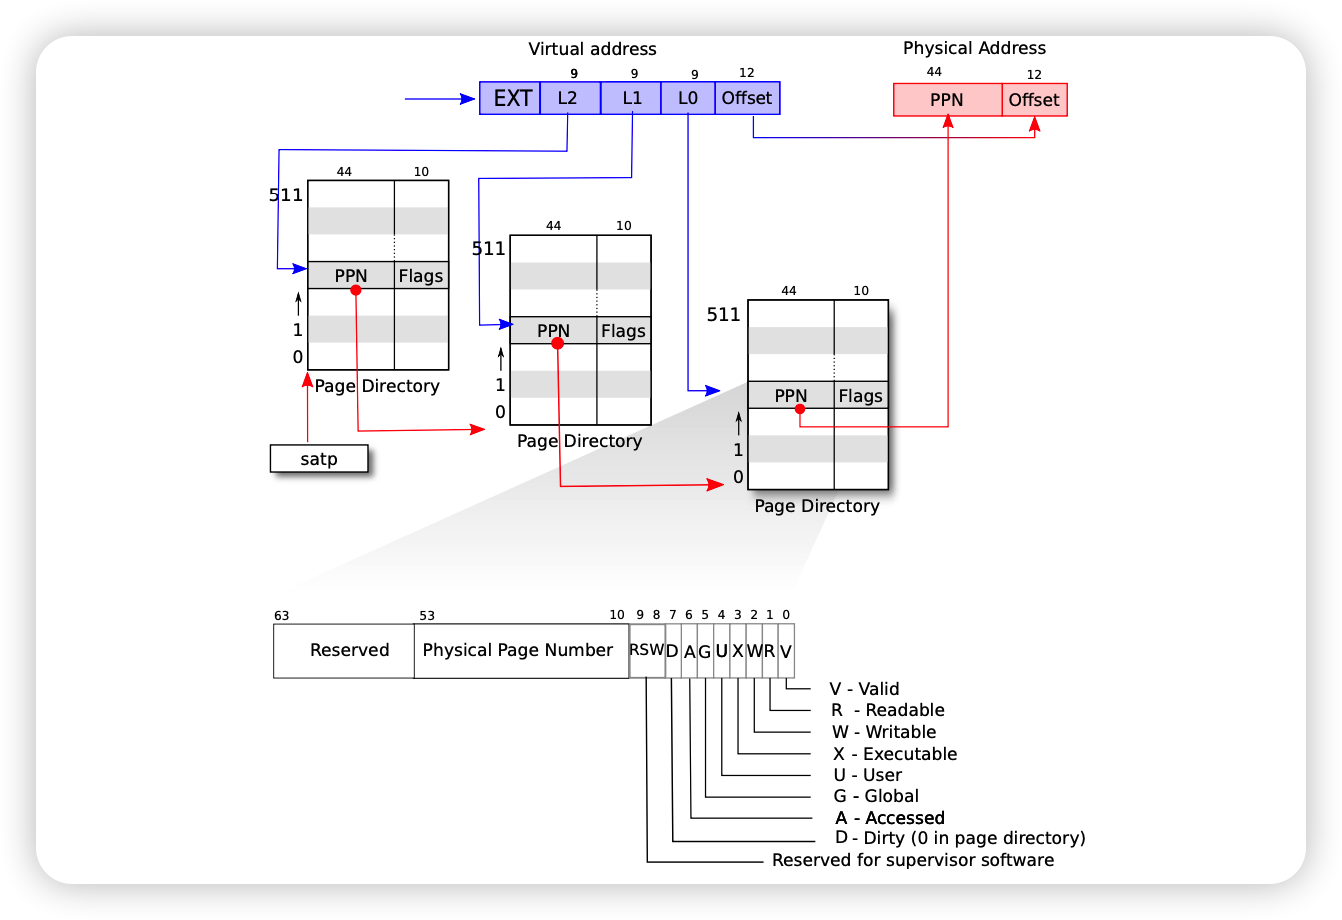
\includegraphics[width=0.8\textwidth]{../imgs/f3-2.png}
    \caption{左侧是xv6的内核地址空间。\texttt{RWX}代表PTE的读、写、执行权限。右侧是xv6期望看到的RISC-V的物理地址空间。}
    \label{f3-3}
\end{figure}

QEMU仿真出的计算机的RAM(物理内存)从物理地址\texttt{0x80000000}开始并至少持续到\texttt{0x88000000},xv6称这个地址为\texttt{PHYSTOP}。
QEMU的仿真也包含I/O设备,例如磁盘。
QEMU以\emph{内存映射(memory-mapped)}控制寄存器的方式把硬件接口暴露给软件,它把设备映射到\texttt{0x80000000}以下的物理内存地址。
内核可以通过读/写特殊的物理地址来和这些设备交互;这样的读/写会和设备硬件而不是RAM进行交互。
\autoref{ch04}会解释xv6怎么和设备交互。

内核使用“直接映射”访问RAM和内存映射设备寄存器,意思是说,把这些资源映射到和物理地址相同的虚拟地址。
例如,内核自身同时位于虚拟地址和物理地址的\texttt{KERNBASE=0x80000000}处。
直接映射简化了读/写物理内存的内核代码。
例如,当\texttt{fork}为子进程分配用户内存时,分配器会返回内存的物理地址,texttt{fork}在把父进程的用户内存拷贝到子进程时可以直接把它用作虚拟地址。

还有一些内核的虚拟地址并不是直接映射:
\begin{itemize}
    \item trampoline页。它被映射到虚拟地址空间的顶部,在用户页表中它也被映射到虚拟地址空间顶部。\autoref{ch04}会讨论trampoline页扮演的角色,但这里我们可以看到一个有趣的页表用例,一个物理页(存储trampoline代码的那个页)在内核的虚拟地址空间中被映射了两次:一次是在虚拟地址空间的顶部,一次是直接映射。
    \item 内核的栈页。每个进程都有自己的内核栈,它被映射到很高的地址处,这样xv6可以在它下面留一个未映射的\emph{保护页(guard page)}。保护页的PTE是无效的(即,\texttt{PTE\_V}位未被设置),这样如果内核溢出了内核栈,它很有可能会触发一个异常,并且内核会崩溃。如果没有守护页,栈溢出时可能会覆盖其他内核内存,导致错误的操作。相对之下崩溃更加可取。
\end{itemize}

尽管内核通过高地址处的映射来使用栈,但使用直接映射的地址也可以访问这些栈。
另一种设计是只使用直接映射,然后使用直接映射地址处的栈。
然而在这种设计中,如果想提供保护页,那么需要取消保护页的虚拟地址映射,否则保护页会映射到物理地址,而这些被取消映射的物理地址将很难再使用起来。

内核以\texttt{PTE\_R}和\texttt{PTE\_X}权限映射trampoline和内核text段的页。
内核将从这些页中读取和执行指令。
内核以权限\texttt{PTE\_R}和\texttt{PTE\_W}映射其他的页面,这样它可以读取和写入那些页面中的内存。
保护页的映射是无效映射。

\section{代码:创建一个地址空间}
xv6中大部分操作地址空间和页表的代码都在\texttt{vm.c}\href{https://github.com/mit-pdos/xv6-riscv/blob/risc/kernel/vm.c#L1}{(kernel/vm.c:1)}中。
其中最主要的数据结构是\texttt{pagetable\_t},它其实是一个指向RISC-V根页表的指针;\texttt{pagetable\_t}要么是内核的页表,要么是进程的页表。
最主要的函数是\texttt{walk}和\texttt{mappages}:\texttt{walk}查找一个虚拟地址对应的PTE,\texttt{mappages}为新的映射添加PTE。
以\texttt{kvm}开头的函数操作内核页表,以\texttt{uvm}开头的函数操作用户页表,其他的函数同时用于两者。
\texttt{copyout}把数据拷贝到用户虚拟地址,\texttt{copyin}相反,地址作为系统调用的参数提供。
它们都在\texttt{vm.c}里,因为它们需要显式地翻译这些地址以找到相应的物理内存。

在启动的早期,\texttt{main}会调用\texttt{kvminit}\href{https://github.com/mit-pdos/xv6-riscv/blob/risc/kernel/vm.c#L54}{(kernel/vm.c:54)},这个函数会使用\texttt{kvmmake}\href{https://github.com/mit-pdos/xv6-riscv/blob/risc/kernel/vm.c#L20}{(kernel/vm.c:20)}创建内核的页表。
这次调用在xv6启用RISC-V的分页功能之前执行,因此其中的地址都直接是物理地址。
\texttt{kvmmake}首先分配一个物理内存页来存储根页表。
然后它调用\texttt{kvmmap}来添加内核翻译地址时需要的映射。
这些映射包括内核的指令和数据、至多到\texttt{PHYSTOP}的物理内存、以及实际上是设备的内存范围。
\texttt{proc\_mapstacks}\href{https://github.com/mit-pdos/xv6-riscv/blob/risc/kernel/proc.c#L33}{(kernel/proc.c:33)}为每个进程分配一个内核栈。
它会调用\texttt{kvmmap}把每个栈映射到\texttt{KSTACK}生成的虚拟地址,以为无效的保护页留出空间。

\texttt{kvmmap}\href{https://github.com/mit-pdos/xv6-riscv/blob/risc/kernel/vm.c#L132}{(kernel/vm.c:132)}会调用\texttt{mappages}\href{https://github.com/mit-pdos/xv6-riscv/blob/risc/kernel/vm.c#L143}{(kernel/vm.c:143)},它把一系列从虚拟地址到物理地址的映射加入到页表中。

\texttt{walk}\href{https://github.com/mit-pdos/xv6-riscv/blob/risc/kernel/vm.c#L86}{(kernel/vm.c:86)}模仿RISC-V的分页硬件查找虚拟地址的PTE的过程(见\autoref{f3-2})。
\texttt{walk}每次用9位逐次查找3级页表。
它使用虚拟地址的每9位去查找下一级页表或者最终目标页的PTE\href{https://github.com/mit-pdos/xv6-riscv/blob/risc/kernel/vm.c#L92}{(kernel/vm.c:92)}。
如果PTE无效,说明请求的页面还没有被分配,如果\texttt{alloc}参数为真,\texttt{walk}会分配一个新的页并把它的物理地址加进PTE里。
它返回树的最底层的PTE的地址\href{https://github.com/mit-pdos/xv6-riscv/blob/risc/kernel/vm.c#L102}{(kernel/vm.c:102)}。

上面的代码依赖于物理内存被直接映射到内核的虚拟地址空间。
例如,\texttt{walk}逐级查询页表时,它从PTE中获取下一级页表的(物理)地址\href{https://github.com/mit-pdos/xv6-riscv/blob/risc/kernel/vm.c#L94}{(kernel/vm.c:94)},然后把它当做一个虚拟地址来获取下一级页表中的PTE\href{https://github.com/mit-pdos/xv6-riscv/blob/risc/kernel/vm.c#L92}{(kernel/vm.c:92)}。

\texttt{main}调用\texttt{kvminithart}\href{https://github.com/mit-pdos/xv6-riscv/blob/risc/kernel/vm.c#L62}{(kernel/vm.c:62)}来安装页表。
它把根页表的物理地址存入\texttt{satp}寄存器。
之后CPU就会使用内核的页表翻译所有的地址。
因为内核使用了直接映射,现在下一条指令的虚拟地址将会映射到正确的物理内存地址。

每一个RISC-V CPU都会页表项缓存到\emph{翻译查找缓冲区(Translation Look-aside Buffer, TLB)}中,所以当xv6修改一个页表时,它必须告诉CPU把相应的缓存的TLB条目无效化。
如果不这么做,之后TLB可能会使用旧的映射,旧的映射可能指向一个现在已经被分配给别的进程的物理页,这样一个进程就可能扰乱其他进程的内存。
RISC-V有一条指令\texttt{sfence.vma}用来清空当前CPU的TLB。
xv6在\texttt{kvminithart}中修改\texttt{satp}寄存器之后执行了\texttt{sfence.vma},trampoline代码中在返回用户空间之前会先切换到用户的页表,之后也要执行\texttt{sfence.vma}\href{https://github.com/mit-pdos/xv6-riscv/blob/risc/kernel/trampoline.S#L89}{(kernel/trampoline.S:89)}。

在修改\texttt{satp}之前执行\texttt{sfence.vma}也是必要的,这是为了等待所有load/store指令的完成。
这可以保证之前对页表的更新已经完成,也确保之前的load和store都是用的旧的页表,而不是新的。

为了避免清空整个TLB,RISC-V CPU可以支持地址空间标识符(ASID)[3]。
这样内核可以只情况特定地址空间的TLB条目。
xv6并没有用到这个feature。

\section{物理内存分配}
内核必须在运行期间为页表、用户内存、内核栈、管道缓冲区分配和释放物理内存。

xv6使用从内核的结尾开始到\texttt{PHYSTOP}之间的物理内存进行运行时分配。
它每次分配和释放一个4096字节的页。
它通过页面本身串联成的链表来持续追踪哪些页面是空闲的。
分配一个页面需要从链表中移除一个页,释放一个页面需要把页加回到空闲链表中。

\section{代码:物理内存分配器}
分配器的代码在\texttt{kalloc.c}\href{https://github.com/mit-pdos/xv6-riscv/blob/riscv//kernel/kalloc.c#L1}{(kernel/kalloc.c:1)}中。
分配器的数据结构是物理内存页组成的\emph{空闲链表(free list)}。
每个空闲页对应的链表节点是一个\texttt{struct run}\href{https://github.com/mit-pdos/xv6-riscv/blob/riscv//kernel/kalloc.c#L17}{(kernel/kalloc.c:17)}。
分配器把这些数据结构存储到何处呢?
它把每个空闲页的\texttt{run}结构体直接存储在这个页里,因为这个页目前是空闲的,所以里面没有别的内容。
空闲链表被一个自旋锁\href{https://github.com/mit-pdos/xv6-riscv/blob/riscv//kernel/kalloc.c#L21-L24}{(kernel/kalloc.c:21-24)}保护着。
列表和锁被包装进一个结构体以清晰地表明这个锁是为了保护结构体中的字段。
目前我们可以忽略这个锁和\texttt{acquire}、\texttt{release}调用,\autoref{ch06}将会详细介绍锁。

\texttt{main}函数会调用\texttt{kinit}来初始化分配器\href{https://github.com/mit-pdos/xv6-riscv/blob/riscv//kernel/kalloc.c#L27}{(kernel/kalloc.c:27)}。
\texttt{kinit}把空闲链表初始化为包含内核结尾到\texttt{PHYSTOP}之间的每个页。
xv6本应该通过解析硬件提供的配置信息来决定有多少物理内存可用。
但实际上xv6直接假设机器有128MB的RAM。
\texttt{kinit}会调用\texttt{freerange},它对范围内的每个页调用\texttt{kfree}把它们加入到空闲链表中。
PTE只能指向一个4096字节对齐的物理地址(即这个地址必须是4096的整数倍),因此\texttt{freerage}使用\texttt{PGROUNDUP}来保证它只释放对齐的物理地址。
分配器起始时是没有内存可以管理的,这些\texttt{kfree}的调用给它提供了内存。

分配器有时会把地址当做整数以对它们进行算术运算(例如,遍历\texttt{freerange}中的所有页),有时又会把地址当作指针来读写内存(例如,把\texttt{run}结构体存储在每个页中),对地址的双重用法是分配器的代码中充满C类型转换的主要原因。
另一个原因是释放和分配操作本质上会改变内存的类型。

\texttt{kfree}函数\href{https://github.com/mit-pdos/xv6-riscv/blob/riscv//kernel/kalloc.c#L47}{(kernel/kalloc.c:47)}首先把要释放的页中的每个字节都置为1。
这会导致在页被释放以后(通过“悬垂指针”)访问它的代码读取到的都是垃圾数据而不是旧的有效的数据,这样也许能帮助这样的代码更快地崩溃。
\texttt{kfree}会把页放在空闲列表的首部:它把\texttt{pa}转换成一个\texttt{struct run}的指针,把空闲列表的旧根节点存储在\texttt{r->next}中,然后让空闲列表的根节点等于\texttt{r}。
\texttt{kalloc}移除并返回空闲列表中的第一个节点。

\section{进程地址空间}
每个进程都有单独的页表,当xv6切换进程时,它也会切换页表。
\autoref{f3-4}相比于\autoref{f2-2}更加详细地展示了进城的地址空间。
一个进程的用户内存从虚拟地址0开始并可以增长到\texttt{MAXVA}\href{https://github.com/mit-pdos/xv6-riscv/blob/riscv//kernel/riscv.h#L360}{(kernel/riscv.h:360)},理论上允许一个进程寻址最多256GB的内存。

\begin{figure}[htbp]
    \centering
    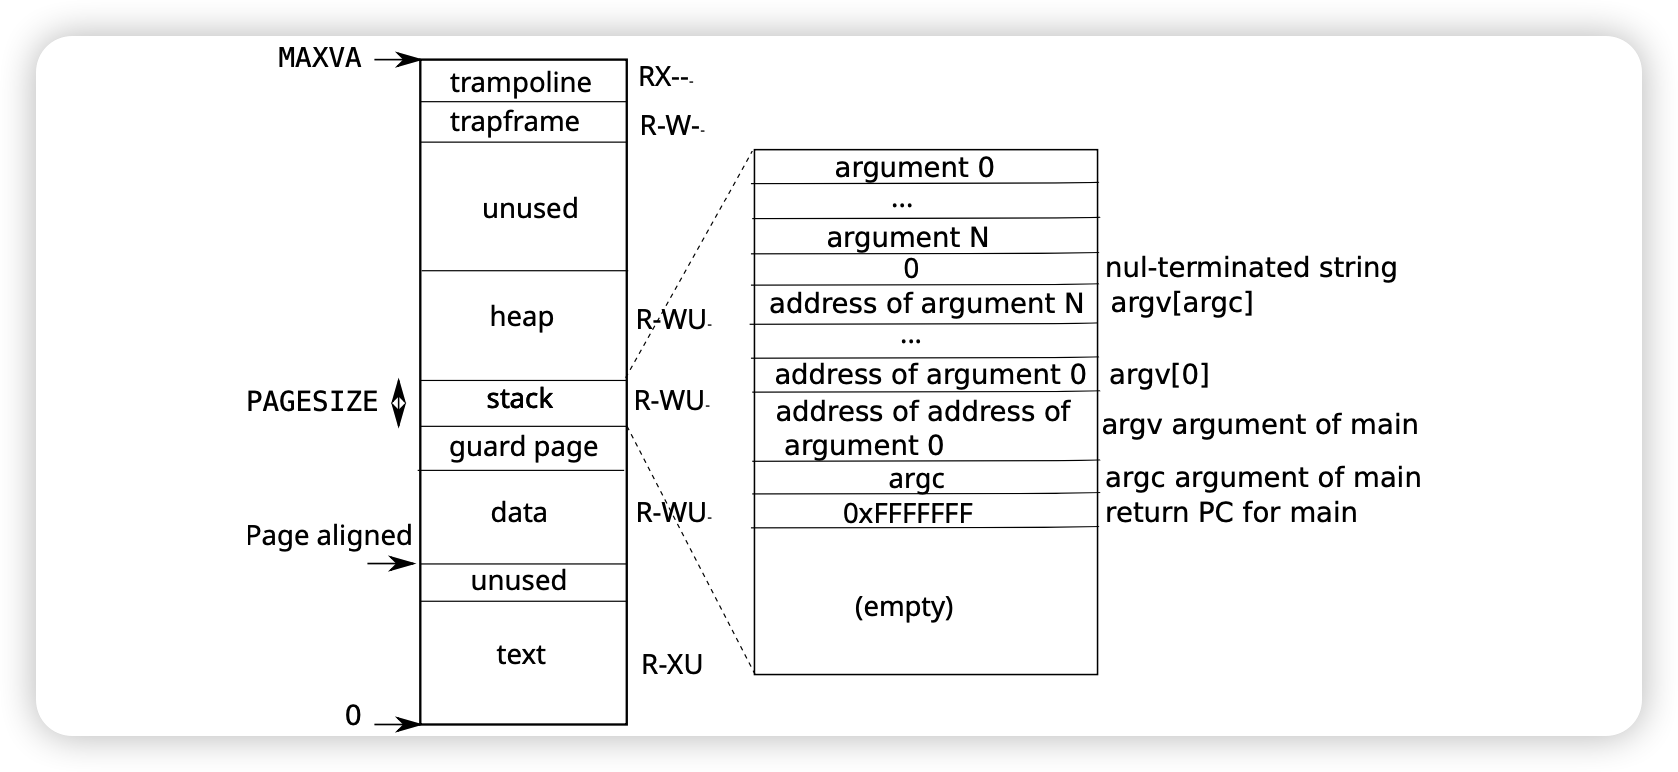
\includegraphics[width=0.8\textwidth]{../imgs/f3-4.png}
    \caption{一个进程的用户地址空间和它的初识栈。}
    \label{f3-4}
\end{figure}

一个进程的地址空间由包含程序代码的页(xv6以权限\texttt{PTE\_R}、\texttt{PTE\_X}、\texttt{PTE\_U}映射这些页)、包含程序中预初始化数据的页、栈的页、堆的页组成。
xv6以权限\texttt{PTE\_R}、\texttt{PTE\_W}、\texttt{PTE\_U}映射数据、栈和堆的页。

在用户地址空间内使用权限是一种通用的保护用户进程的技术。
如果代码被以\texttt{PTE\_W}映射,那么一个进程可能会偶然间修改它里面的程序。
例如,一个编程错误可能会导致程序写入空指针,这回修改地址0处的指令,然后再继续运行,可能会导致更大的问题。
为了立刻检测出这种错误,xv6映射代码时并不赋予\texttt{PTE\_W}权限,如果一个程序偶然尝试写入地址0,硬件会拒绝执行并抛出一个页面错误(见\autoref{s4-6})。
然后内核会杀死这个进程并打印出一条有用的信息,以帮助程序员定位这个问题。

与此类似,在映射数据时并不赋予\texttt{PTE\_X}权限,这样一个用户程序不可能偶然跳转到数据部分的某个地址并当成指令执行。

在真实世界中,仔细设置权限来保护过程也有助于抵御安全攻击。
一个攻击者可能会把精心设计的输入发给程序(例如,一个web服务器),然后触发程序中的bug,希望把这个bug转换成一个漏洞[14]。
仔细设置权限和一些其他的技术(例如随机化用户地址空间的布局)可以增大这样的攻击的难度。

栈只有单个页,并有一些由\texttt{exec}创建的初始内容。
包含命令行参数的字符串和一些指向它们的指针位于栈的顶部。
再往下是一些允许程序从\texttt{main}开始执行的值,就像刚刚调用函数\texttt{main(argc, argv)}一样。\footnote{todo!}

为了检测用户栈溢出分配好的栈内存,xv6通过清除\texttt{PTE\_U}标记在栈下面放了一个不可访问的守护页。
如果用户栈溢出了并且进程尝试使用栈下面的地址,硬件会生成一个页面错误异常,因为守护页对用户模式下运行的程序来说是不可访问的。
一个真实世界中的操作系统可能会在栈溢出时自动为它分配更多的内存。

当一个进程向xv6要求更多用户内存时,xv6会增长进程的堆。
xv6首先使用\texttt{kalloc}来分配物理页。
然后向进程的页表中添加一个指向新物理页的PTE。
xv6为这些PTE设置了\texttt{PTE\_W}、\texttt{PTE\_R}、\texttt{PTE\_U}、\texttt{PTE\_V}标记。
大部分进程不会使用到整个用户地址空间,xv6会保持未使用的PTE中不设置\texttt{PTE\_V}标记。

这里我们看到了一些使用页表的例子。
首先,不同进程的页表把用户地址翻译到不同的物理内存页,这样每个进程都有私有的用户内存。
其次,每个进程都把它的内存看作从0开始的连续虚拟地址,而进程的物理内存可以是不连续的。
然后,内核把trampoline代码的页映射到用户地址空间的顶部(没有\texttt{PTE\_U}),这样一个物理页就可以在所有地址空间中可见,但只有内核可以使用它。

\section{代码:\texttt{sbrk}}
\texttt{sbrk}是一个系统调用,进程可以使用它缩减或增长自己的内存。
这个系统调用由函数\texttt{growproc}\href{https://github.com/mit-pdos/xv6-riscv/blob/riscv//kernel/proc.c#L260}{(kernel/proc.c:260)}实现。
\texttt{growproc}可能会调用\texttt{uvmalloc}或\texttt{uvmdealloc},取决于\texttt{n}是正数还是负数。
\texttt{uvmalloc}\href{https://github.com/mit-pdos/xv6-riscv/blob/riscv//kernel/vm.c#L226}{(kernel/vm.c:226)}使用\texttt{kalloc}分配内存,并使用\texttt{mappages}向用户页表中添加PTE。
\texttt{uvmdealloc}会调用\texttt{uvmunmap}\href{https://github.com/mit-pdos/xv6-riscv/blob/riscv//kernel/vm.c#L171}{(kernel/vm.c:171)},它使用\texttt{walk}寻找PTE并使用\texttt{kfree}释放它们指向的物理内存。

xv6使用进程的页表时,不仅是用它来告诉硬件如何映射用户虚拟地址,还用它来记录哪些物理内存页已经被分配给进程。
这样是为什么释放用户内存(在\texttt{uvmunmap}中)需要检查用户页表。

\section{代码:\texttt{exec}}
\texttt{exec}系统调用把进程的用户地址空间替换为一个(二进制/可执行文件)文件的内容。
二进制文件通常是编译器和链接器输出的文件,它包含机器指令和程序的数据。
\texttt{exec}\href{https://github.com/mit-pdos/xv6-riscv/blob/riscv//kernel/exec.c#L23}{(kernel/exec.c:23)}用\texttt{namei}\href{https://github.com/mit-pdos/xv6-riscv/blob/riscv//kernel/exec.c#L36}{(kernel/exec.c:36)}打开二进制文件\texttt{path},\texttt{namei}将会在\autoref{ch08}中解释。
然后它首先读取ELF头。
xv6的二进制格式是被广泛使用的\emph{ELF格式},在\href{https://github.com/mit-pdos/xv6-riscv/blob/riscv//kernel/elf.h}{(kernel/elf.sh)}中定义。
一个ELF二进制程序由ELF头、\texttt{struct elfhdr}\href{https://github.com/mit-pdos/xv6-riscv/blob/riscv//kernel/elf.h#L6}{(kernel/elf.h:6)}、紧随其后的一些程序节头、\texttt{struct proghdr}\href{https://github.com/mit-pdos/xv6-riscv/blob/riscv//kernel/elf.h#L25}{(kernel/elf.h:25)}组成。
每一个\texttt{progvhdr}描述了应用的一个要被加载到内存中的节。
xv6程序有两个程序节:一个用于指令,一个用于数据。

之后首先要快速检查这个文件是否可能包含一个ELF二进制程序。
一个ELF二进制程序由四个字节的“魔数”开头:\texttt{0x7F}、\texttt{'E'}、\texttt{'L'}、\texttt{'F'},或者叫\texttt{ELF\_MAGIC}\href{https://github.com/mit-pdos/xv6-riscv/blob/riscv//kernel/elf.h#L3}{(kernel/elf.h:3)}。
如果ELF头有正确的魔数,\texttt{exec}会假设这个二进制程序的格式是正确的。

\texttt{exec}使用\texttt{proc\_pagetable}\href{https://github.com/mit-pdos/xv6-riscv/blob/riscv//kernel/exec.c#L49}{(kernel/exec.c:49)}创建一个新页表,使用\texttt{uvmalloc}\href{https://github.com/mit-pdos/xv6-riscv/blob/riscv//kernel/exec.c#L65}{(kernel/exec.c:65)}为每个ELF段分配内存,并使用\texttt{loadseg}\href{https://github.com/mit-pdos/xv6-riscv/blob/riscv//kernel/exec.c#L10}{(kernel/exec.c:10)}把每个段加载到内存中。
\texttt{loadseg}使用\texttt{walkaddr}查找到新分配的内存的物理地址,然后写入ELF段的每个页,使用\texttt{readi}来读取文件内容。

\texttt{exec}创建的第一个用户程序是\texttt{/init},它看起来像这样:
\begin{blacklisting}
    # objdump -p user/_init
    user/_init:     file format elf64-little
    Program Header:
    0x70000003 off    0x0000000000006bb0 vaddr 0x0000000000000000
                                           paddr 0x0000000000000000 align 2**0
             filesz 0x000000000000004a memsz 0x0000000000000000 flags r--
        LOAD off    0x0000000000001000 vaddr 0x0000000000000000
                                           paddr 0x0000000000000000 align 2**12
             filesz 0x0000000000001000 memsz 0x0000000000001000 flags r-x
        LOAD off    0x0000000000002000 vaddr 0x0000000000001000
                                           paddr 0x0000000000001000 align 2**12
             filesz 0x0000000000000010 memsz 0x0000000000000030 flags rw-
       STACK off    0x0000000000000000 vaddr 0x0000000000000000
                                           paddr 0x0000000000000000 align 2**4
             filesz 0x0000000000000000 memsz 0x0000000000000000 flags rw-
\end{blacklisting}

我们可以看到text段的内容从文件的0x1000偏移处开始,应该加载到虚拟地址0x0处(没有写权限)。
我们还看到data段应该被加载到虚拟地址0x1000处,这个地址是页的边界,没有执行权限。

一个程序节头中的\texttt{filesz}可能会小于\texttt{memsz},差值表示这些空间应该用0填充(为C的全局变量预留空间)而不是从文件中读取。
对于\texttt{/init},数据段的\texttt{filesz}是0x10字节,而\texttt{memsz}是0x30字节,因此\texttt{uvmalloc}会分配0x30字节的物理内存,但只从\texttt{/init}文件中读取0x10字节。

现在\texttt{exec}该分配并初始化用户栈了。
\texttt{exec}逐个把参数字符串拷贝到栈顶,在\texttt{ustack}中记录下指向它们的指针。
它在传给\texttt{main}的\texttt{argv}数组的末尾放上一个空指针。
\texttt{ustack}中的前三项是虚构的返回地址的程序计数器、\texttt{argc}、\texttt{argv}指针\footnote{译者注:这一句应该是作者笔误,因为这个函数里并没有把这三个东西存进\texttt{ustack}里。去翻了一下x86版的xv6,发现是有这么三行的:\url{https://github.com/mit-pdos/xv6-public/blob/master/exec.c\#L82},应该是作者在编写risc-v版的本书的时候忘了删除这一句。}。

\texttt{exec}会在栈的页下面放一个不可访问的页,这样那些尝试使用超过一个页的程序就会失败。
这个不可访问的页还让\texttt{exec}可以处理过大的参数,这种情况下当\texttt{exec}使用\texttt{copyout}\href{https://github.com/mit-pdos/xv6-riscv/blob/riscv//kernel/vm.c#L352}{(kernel/vm.c:352)}函数把参数拷贝到栈里时,会发现目标的页不可访问,因此会返回-1。

在准备新内存镜像的过程中,如果\texttt{exec}检查到错误,例如无效的程序段,它会跳转到\texttt{bad}标签,释放新的镜像并返回-1。
\texttt{exec}必须等到能确保这一次系统调用将会成功时才能释放旧镜像:因为如果旧镜像已经被释放了,那么这个系统调用就不能向它返回-1了。
\texttt{exec}中只有创建镜像的过程中可能出现错误。
一旦镜像完成,\texttt{exec}可以提交新的页表\href{https://github.com/mit-pdos/xv6-riscv/blob/riscv//kernel/exec.c#L125}{(kernel/exec.c:125)}并释放旧的页表\href{https://github.com/mit-pdos/xv6-riscv/blob/riscv//kernel/exec.c#L129}{(kernel/exec.c:129)}。

\texttt{exec}把ELF文件的内容加载到ELF文件中指定的地址处。
用户或者程序可能会在ELF文件中指定任意地址。
所以\texttt{exec}是有风险的,因为ELF文件中的地址可能会偶然或者故意地指向内核。
如果内核不够谨慎可能会导致崩溃或者被恶意破坏隔离机制(例如,一个安全漏洞)。
xv6进行了很多检查来避免这些风险。
例如\texttt{if (ph.vaddr + ph.memsz < ph.vaddr)}检查求和之后是否溢出64位的整数。
这里的危险在于用户可能会构造出这样一个ELF文件:让\texttt{ph.vaddr}指向一个用户指定的地址,然后让\texttt{ph.memsz}非常大,两者之后可能会溢出到0x1000处,这种情况看起来很像是有效的值。
在xv6的一个旧版本中用户地址空间也包含内核(但在用户模式下不可读/写),用户可能会选择一个对应内核内存的地址,然后从ELF二进制文件中拷贝数据到内核中。
在xv6的RISC-V版本中不可能发生这种情跨过你,因为内核有它自己单独的页表,\texttt{loadseg}把段加载到进程的页表中,而不是内核的页表中。

内核的开发者很容易遗漏关键的检查,真实世界中的内核也有很长一段时间因为缺少检查而被用户程序利用以非法获取内核的特权。
xv6可能无法完全验证提供给内核的用户级数据,恶意用户程序可能能够利用这些数据来规避xv6的隔离。

\section{真实世界}
和大多数操作系统一样,xv6使用分页硬件来进行内存的保护和映射。
大多数操作系统通过组合分页和页面故障异常远比xv6更好地利用分页,我们将在\autoref{ch04}中介绍。

xv6的内核在虚拟和物理地址之间使用了直接映射,并假设有从0x8000000地址处开始的物理RAM,然后把内核加载到这个地址,这大大简化了xv6.
对QEMU来说,这可以正常工作,但在真实的硬件上这是一个坏主意,真实的硬件会把RAM和设备放在一个无法预料的物理地址,因此(例如)0x8000000处可能没有RAM,而xv6期望把内核加载到这个地址。
大多数现实世界中的内核设计会利用页表把任意的硬件物理内存布局转换为可预料的内核虚拟地址布局。

RISC-V支持在物理地址的层面保护内存,但xv6并不会用到这个功能。

在有很多内存的机器上,使用RISC-V对“超级页(super page)”的支持可能会很有用。
当物理内存很小时使用小页面会更好,这样可以支持细粒度地分配页面和把页面换出到磁盘。
例如,如果一个程序只使用8KB的内存,给它一个4MB大小的超级页内存是很浪费的。
更大的页面适合有很多RAM的机器,可以减少页表处理的开销。

xv6的内核缺少一个类似\texttt{malloc}一样的可以为更小的对象分配内存的分配器,这让内核
无法使用需要动态分配内存的复杂数据结构。
一个更精密的内核应该能分配很多任意大小的小内存块,而不是(像xv6一样)只能分配4096字节的块。
一个真正的内核分配器既要能处理小内存块的分配,也要能处理大内存块的分配。

内存分配一直都是一个热门话题,基本的问题是高效地利用有限的内存和为未来未知的请求做好准备[9]。
如今相比起空间效率,人们更关心速度。

\section{练习}


